\chapter{Descriptors extraction}
In person re-identification, it's very important to choose robust descriptor to represent person. A good descriptor should be robust to variations of illumination, viewpoint, and camera color response. Most descriptors tries to seize the color and texture information. In this chapter, we will first introduce some basic descriptors and compare their performance on VIPeR dataset, then a detailed introduction of hierarchical descriptor will be presented in the coming section.


\section{Color and textural features}
\subsection{Color histogram descriptors on different color space}
Histogram descriptor extracts color statistics information of input images. A popular histogram extracting method is to divide input image into a few horizontal stripes and extract color histogram of each stripe, then they are concatenated to consist of histogram descriptor of the whole image. Color space selection has much influence on descriptor performance. HSV color space is very common in computer vision and image processing area for target detection and tracking. The HSV descriptor has better performance than RGB histogram descriptor[] since HSV color separates image intensity from color information. Thus HSV color space is more robust to illumination variation. An unsupervised CMC performance comparison among different color spaces on VIPeR dataset is given in figure []. In this comparison camera a views are used as probe set and camera B views are used for gallery set. We can find that those color spaces separating intensity information outperform RGB color space and HSV outperforms all other color spaces.
%-----------------------------------------------------------------------------

\begin{figure}[H]
\centering
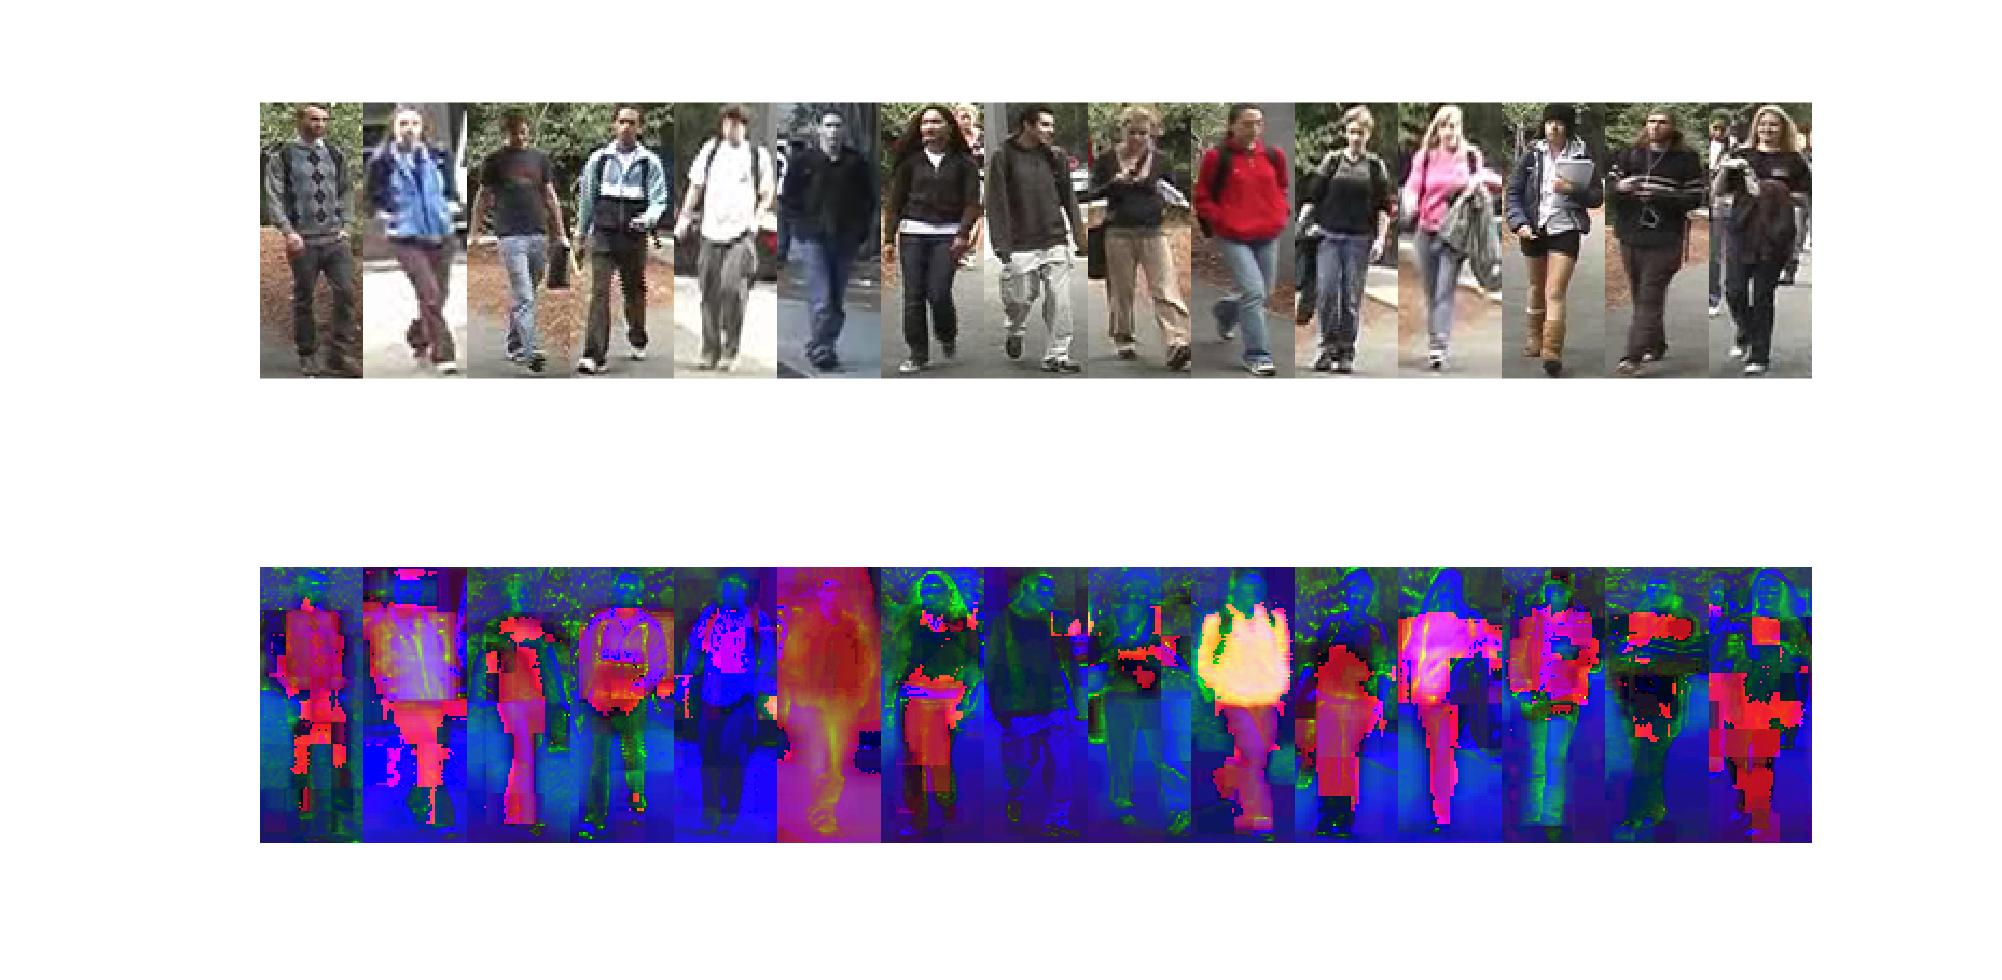
\includegraphics[width=1\linewidth]{/Users/JohnsonJohnson/Downloads/thesis_1/Figures/CompRGBHSV.jpg}
\caption{RGB and HSV visual comparison, the first row is RGB and second row is HSV for same views }
\vspace{0em}
\end{figure} 

\begin{figure}
\centering

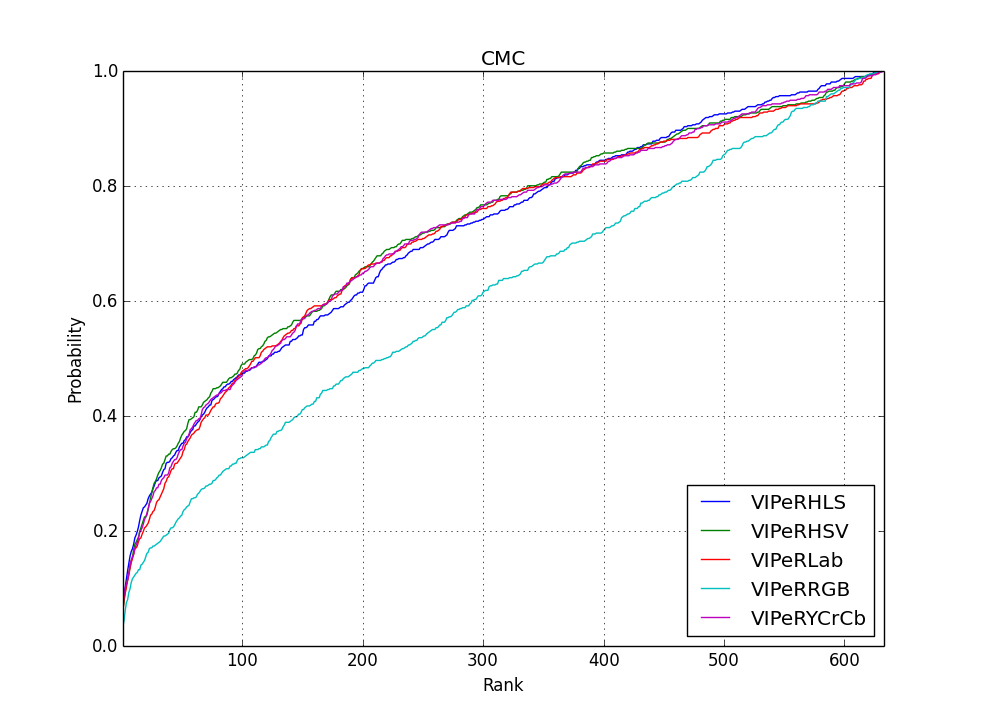
\includegraphics[width=1\linewidth]{/Users/JohnsonJohnson/Downloads/thesis_1/Figures/DifferentColorspaceCMCVIPeR.png}
\caption{A CMC comparison of color histogram on different color spaces }
\vspace{0em}
\end{figure} 
%-----------------------------------------------------------------------------

\textbf{Analysis of histogram based descriptor} The performance of histogram descriptors suffers from ignoring the spatial information. Since it doesn't consider the relative distribution of color, images with same kind color patches but different distribution may have the same histogram descriptor. One example is shown in figure [].

\begin{figure}[H]
\begin{minipage}[t]{0.5\linewidth}
\centering
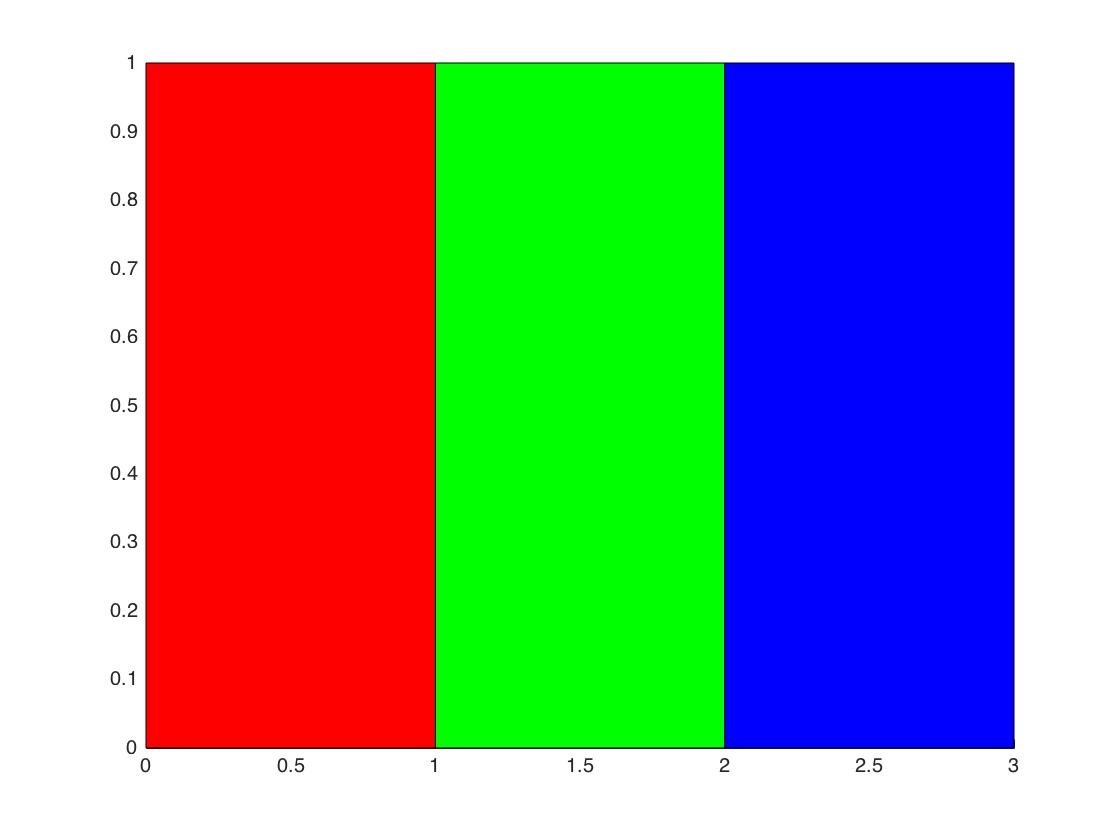
\includegraphics[width=2.2in]{/Users/JohnsonJohnson/Downloads/thesis_1/Figures/RGB.jpg}
%\caption{RGB patch}
\label{fig:side:a}
\end{minipage}%
\begin{minipage}[t]{0.5\linewidth}
\centering
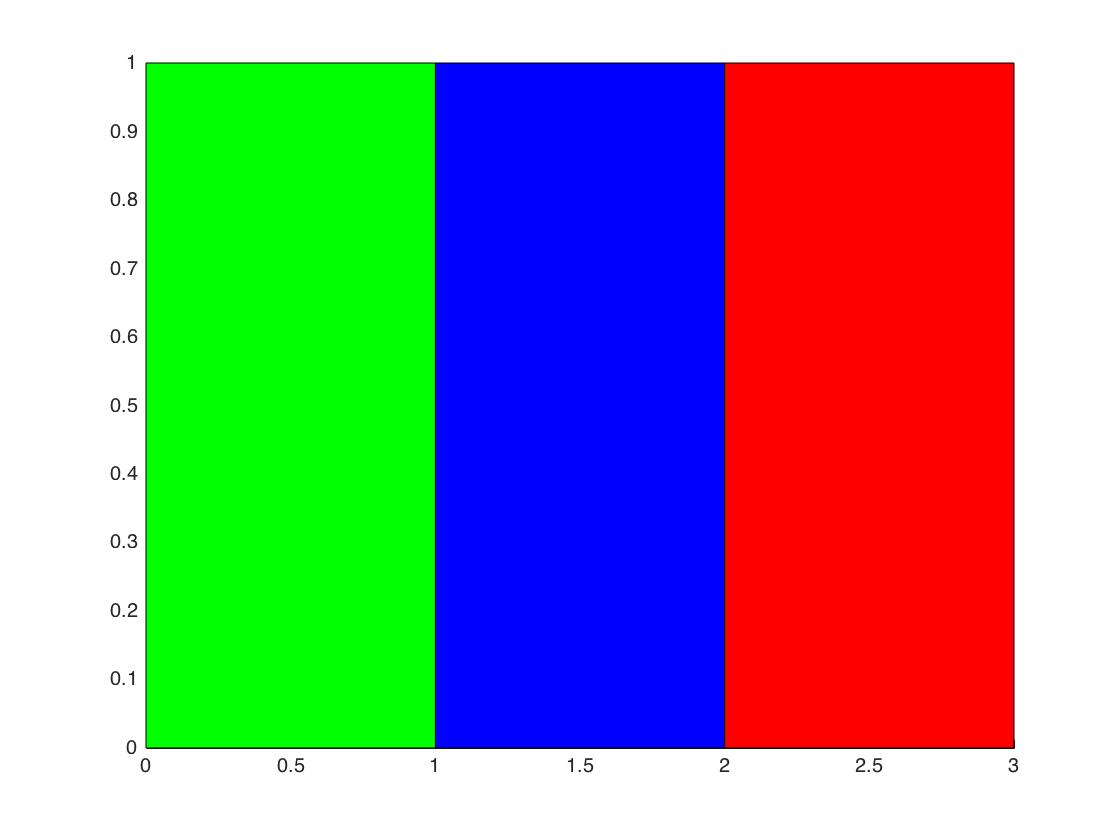
\includegraphics[width=2.2in]{/Users/JohnsonJohnson/Downloads/thesis_1/Figures/GBR.jpg}
%\caption{GBR patch}
\label{fig:side:b}
\end{minipage}
\caption{A comparison of two patches with same entropy but different color distribution}
\end{figure}

\subsection{Local binary pattern(LBP)}
Local binary pattern[] extracts the texture information with efficient computing and has been used on people detection and recognitions. Figure [] is an example of LBP example. by thresholding neighbour pixel of center pixel, the pixels are transformed into a binary integer. There are many variants of LBP like circular LBP, 
LBP is well known for its robustness to monotonic illumination variation.
\begin{figure}[H]
\centering
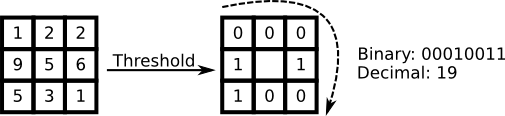
\includegraphics[width=0.8\linewidth]{/Users/JohnsonJohnson/Downloads/thesis_1/Figures/LBPdemo.png}
\caption{An LBP example, by thresholding the neighbour pixels the pixels are transformed into a binary number }
\vspace{0em}
\end{figure}

\subsection{Histogram of oriented gradients(HOG)}
The HOG descriptor extracts textural information of input. 



\section{Influence of background segmentation on different descriptors}
Many works try to minimize impact of background noise of pedestrians' image. It's easier to automatically segment foreground from sequential videos than a single frame. In [SDALF] the author provides foreground mask for all images.  Some of those segmented foreground are shown in figure [] and it's obvious that certain bogy parts like head and feet are lost. To compare those loss's impact on color and textural descriptors, a comparison of foreground segmentation on HSV color histogram descriptors and local binary pattern(LBP) is given in figure [] and figure []. 


\begin{figure}[H]
\centering
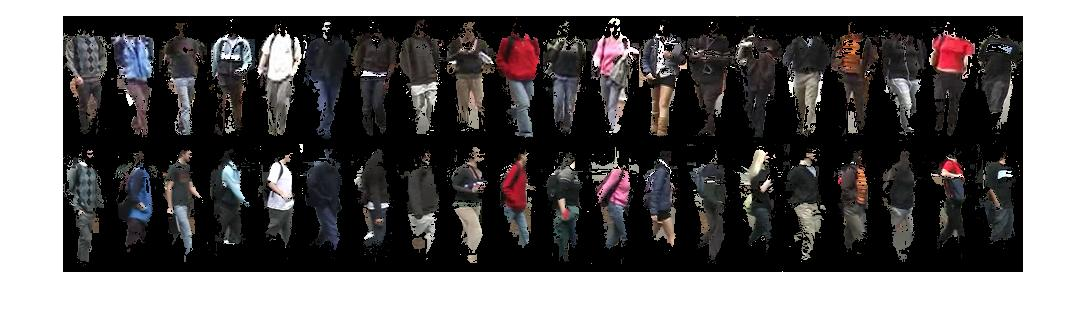
\includegraphics[width=1\linewidth]{/Users/JohnsonJohnson/Downloads/thesis_1/Figures/FGdemo2VIPeR.jpg}
\caption{Foreground segmentation of individuals from VIPeR }
\vspace{0em}
\end{figure} 

We can find that foreground segmentation decreases LBP's performance onVIPer dataset but increases HSV color histogram greatly. The reason for this is imperfect foreground segmentation causes body parts(like head and feet) loss and small black patches in torso and legs, and for some individuals a part of background scene is regarded as foreground. Since HSV color histogram doesn't handle spatial distribution but only color entropy, foreground segmentation improves its performance greatly. But since LBP handles texture for each sample patch, its performance suffers from those body parts loss and those little black patches. 

\begin{figure}[H]
\centering

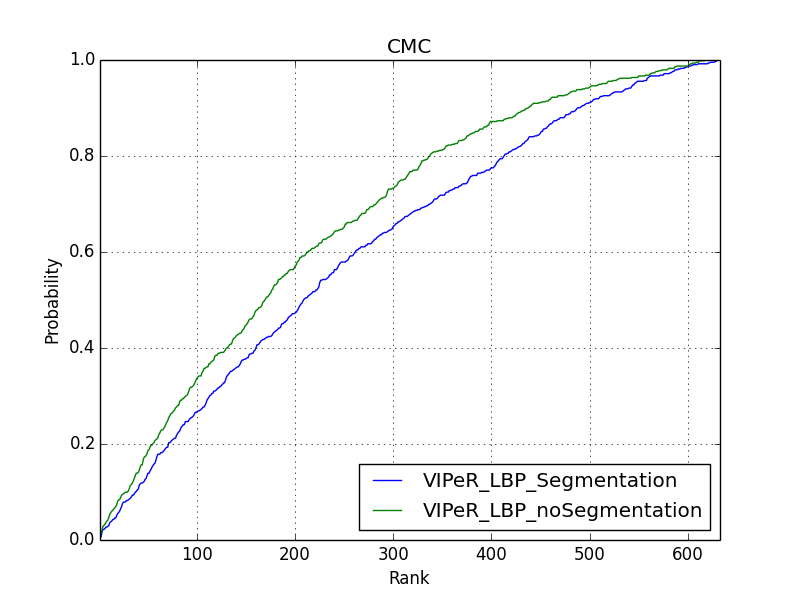
\includegraphics[width=1\linewidth]{/Users/JohnsonJohnson/Downloads/thesis_1/Figures/VIPeR_LBP_FGSegComparison.png}
\caption{A CMC comparison of foreground segmentation on LBP tested on VIPeR }
\vspace{0em}
\end{figure} 

\begin{figure}[H]
\centering
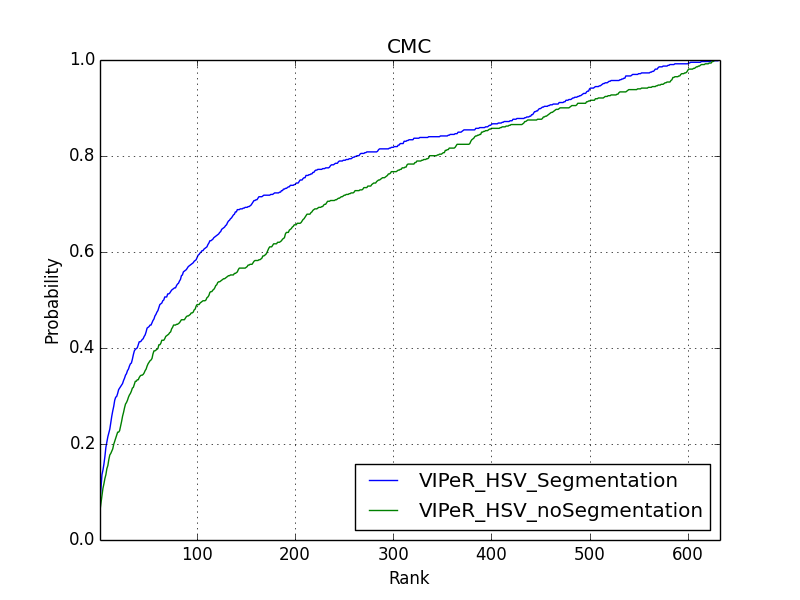
\includegraphics[width=1\linewidth]{/Users/JohnsonJohnson/Downloads/thesis_1/Figures/VIPeR_FG_HSV_comparison.png}
\caption{A CMC comparison of foreground segmentation on HSV histogram descriptor tested on VIPeR}
\vspace{0em}
\end{figure} 


\section{The hierarchical gaussian descriptor}

The hierarchical gaussian descriptor is proposed by in  \cite{GOGpaper}, this descriptor uses a two-level gaussian distribution to model an individual. This descriptor densely sample the image and model each hierarchical structure with gaussian distribution and has outperformed many other works. Firstly it divides the image into a few overlapping horizontal slides, and in each slide, dense sampling patches are made with certain size. So there is a  two-level structure in this image, small patches and slides. Then by model each level with gaussian model we can get a robust representation of the individual.
\subsection{Single pixel modelling}

In this hierarchical model, it is very important to have a full representation for every single pixel. To fully characterize single pixel, a $d$ dimensional vector is used to represent it. In this vector, there could be any predefined properties like coordinates, color values, texture and filter response. Suppose the original image is in RGB color space, the gaussian of gaussian descriptor uses a 8-dimensional vector $\textbf{f}$, and 
$\bm{f}_i = (y,M_0,M_{90},M_{180},M_{270},R,G,B)$.
The y component is the y coordinate of pixel, and $M_{\{{\theta}\in{0^o,90^o,180^o,270^o}\}}$ is the quantized gradient information in 4 directions. The last three component is the color value is specified color space.

In all the benchmark dataset, all the images are cropped with a bounding box well suited the individual, and the pedestrian in an image can be at left or right of center, while in the vertical direction the head and feet of pedestrian is very close the image edge. So for each pixel, the y coordinate is more correlated than x coordinate, so only y coordinate is chosen for pixel modelling. 

Then the $M$ is to characterize the texture with the gradient histogram. Different $M$ values is the magnitude of gradient in every direction. 
Firstly the gradient in x and y direction are computed by two gradient filters $\rm{h}_x$ and $\rm{h}_y$, and we have 
\begin{equation}
\begin{aligned}
h_x = [-1, 0, 1]\\
h_y = -h_x'
\end{aligned}
\end{equation}

Then by convolve those two filters with the intensity image $I$, the horizontal and vertical gradient $I_x, I_y$ can be computed, so the orientation and magnitude can be computed by following equations:
\begin{equation}
\begin{aligned}
O(i,j) = (\arctan(I_y(i,j)/I_x(i,j))+\pi)*180 /{\pi} \\
M(i,j) = \sqrt{(I_x(i,j)^2 + I_y(i,j))^2}
\end{aligned}
\end{equation}

The orientation are quantized into four bins by a soft voting algorithm[ GOG15]. For each pixel its corresponding gradient orientation is decided by its nearest bin's direction. To make the descriptor focus on the gradient components with high values, the gradient and orientation are multiplied as follow,
\begin{equation}
M_{\theta} = MO_{\theta},
\end{equation}

%For every gradient magnitude value with its orientation , the corresponding weights of all predefined directions are computed, and the direction with the biggest weight is chosen as the quantized direction for this pixel.

To model the patch with a multi-variate gaussian distribution, we have to estimate its mean value and the covariance matrix. A multi-variate gaussian model has the form
\begin{equation}
G(\bm{f}_i;\bm{\mu},\bm{\Sigma}) = \frac{\exp^{(\frac{1}{2}(\bm{f}-\bm{\mu})^T\bm{\Sigma}^{-1}(\bm{f}-\bm{\mu}))}}{(2\pi)^{d/2}|{\bm{\Sigma|}}} 
\end{equation}

where $\bm {\mu}$ is the estimated mean value, and $\bm {\Sigma} $ is the estimated covariance matrix. 

To estimate the parameters for this gaussian model based on sampled patches pixel features, the maximal likelihood estimate(MLE) is used. According MLE algorithm, we have the following estimated parameters
\begin{equation}
%\begin{aligned}
\bm{\mu} = \frac{1}{n}\sum \bm{f}_i,
%\end{aligned}
\end{equation}
\begin{equation}
%\begin{aligned}
\bm{\Sigma} = \frac{1}{n-1} (\bm{f}_i-\bm{\mu})(\bm{f}_i-\bm{\mu})^T,
%\end{aligned}
\end{equation}

where $n$ is the number of pixels in current patch. When the gaussian model is computed, the next step is to model all the patch gaussians. But it's a complex problem to directly model those multivariate gaussian functions. So some transformation will be operated on estimated parameters $\mu$ and $\Sigma$.

%%Integral image for fast computing
\subsection{Integral image for fast computation}

To compute the estimated covariance matrix $\Sigma$, the integral image is used to reduce time complexity. The integral image[ ] is a intermediate representation to fast compute rectangle area sum in an image. Each pixel value in integral image is the sum of all the pixels inside the rectangle bounded by current pixel and the upper left pixel. That is, the integral image S(x, y) for image I(x, y) is 
\begin{equation}
S(x', y') = \sum_{x<x', y <y'} I(x, y),
\end{equation}

\begin{figure}[H]
\centering
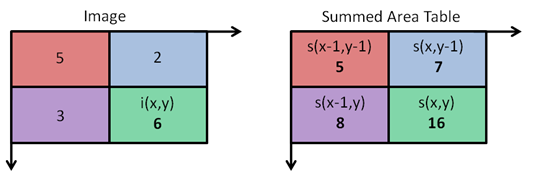
\includegraphics[width=1\linewidth]{/Users/JohnsonJohnson/Downloads/thesis_1/Figures/IntegralImage.png}
\caption{Integral image}
\vspace{0em}
\end{figure} 



%% --------------------------------------Riemannian manifold based SPD transformation
\subsection{Riemannian manifold based SPD transformation}

As described before this hierarchical gaussian descriptor is a stochastic feature, so operations like computing mean and covariance need to be operated on previous summarized gaussian distributions. Mean and covariance operation in Euclidean space can not be directly finished on previous estimated gaussian functions. A transformation is needed to make stochastic summarization feasible on previous level function.
In fact, the multivariate gaussian model is a Riemannian manifold and can be embedded into a semi positive definite matrix(SPD) space. The gaussian function is mapped into a vector space with two steps mapping. A $d$ dimensional multivariate gaussian function can be mapped into a $d+1$ dimensional $SPD_+$ space. According to [GOG25], the mapping can be denoted as 
\begin{equation}
G(\bm{x}_i;\bm{\mu}_i,\bm{\Sigma}_i) \sim \bm{P}_i  = |\bm{\Sigma}_i|^{1/(d+1)} \left[ \begin{matrix}
\bm{\Sigma}_i + \bm{\mu}_i\bm{\mu}^T & \bm{\mu}_i \\
\bm{\mu}_i^T & 1
\end{matrix}
\right]
\end{equation}
The covariance matrix $\bm{\Sigma}_i$ can be singular for small number of pixels within the patch, to avoid this problem a regular factor $\lambda$ is added to $\bm{\Sigma}_i$ so that $\bm{\Sigma}_i = \bm{\Sigma}_i + \lambda\bm{I}$. 

After this mapping, the $n+1$ dimensional SPD matrix needs to be transformed as a vector. The matrix logarithm is used to transform it to tangent space. A $d+1$ dimensional SPD matrix can be mapped as a $d*(d+3)/2+1$ vector, which can be denoted as $SPD_i^+ \sim \bm{p}_i = vec(log(\bm{P}_i))$. Since $\bm{P}_i$ is a positive symmetric matrix?and it can be compressed by half that only the upper triangular 
elements are preserved. To ensure the sum of norm-1 remain the same after compression, the magnitude of off-diagonal elements in $\bm{P}_i$ are timed by $\sqrt2$.  Let $\bm{Q}=\log{\bm{P}_i}$, we have
\begin{equation}
%\begin{aligned}
 \bm{p}_i = [\bm{Q}_{1,1},\sqrt2\bm{Q}_{1,2},\sqrt2\bm{Q}_{1,3},\cdots,\sqrt2\bm{Q}_{1,d+1},
 \end{equation}
 \begin{equation}
 \bm{Q}_{2,2},\sqrt2\bm{Q}_{2,3,},\cdots,\sqrt2\bm{Q}_{2,d+1,},\cdots,\bm{Q}_{d+1,d+1,}]
%\end{aligned}
\end{equation}

With the Gaussian parameters extracted in each region, the same transformation is operated on them. Then all horizontal slides' descriptor are concatenated to get the whole descriptor for the whole image.

\textbf{Dimension analysis} It has been shown in [ ]  combination of descriptors of different color space can greatly improve re-ID performance. In this project, the hierarchical gaussian descriptor in RGB color space is the base descriptor. Descriptors in three more color space \{HSV, Lab, nRGB\}is extracted. The nRGB color space is calculated as 
\begin{equation}
\begin{aligned}
nR = \frac{R}{R+G+B},\\
nG = \frac{G}{R+G+B},\\
nR = \frac{B}{R+G+B}, 
\end{aligned}
\end{equation}

since $nB$ can be calculated with $nR$ and $nG$, in this color space only the first two channel values are used to reduce redundancy. Therefore, for color space \{RGB, HSV, Lab, nRGB\}, the corresponding dimension of pixel feature is \{8, 8, 8, 7\}. After the matrix to vector transformation, the dimension of patch gaussian vector of each channel is \{45, 45, 45, 36\}. Again after the patch gaussian to region gaussian transformation, the dimension of each channel is \{1081, 1081, 1081, 703\}. Suppose there are 7 horizontal slides in each image, the dimension of concatenated descriptor of each channel is \{7567, 7567, 7567, 4921\}. If four color space are all used, the dimension is the sum of each channel as 27622. 





